\chapter{Métodos Utilizados}\label{ch:metodos}
Este capítulo descreve a metodologia aplicada no desenvolvimento do trabalho, que tem como objetivo uma solução para dispositivos móveis para a realização de experimentos das atividades enzimáticas do solo. Para realizar o trabalho foram utilizados os conceitos de engenharia de requisitos como parte inicial do projeto, a modelagem do sistema por meio de requisitos funcionais e casos de uso, e a definição dos processos de desenvolvimento do software que serão apresentados nas próximas seções.

\section{Análise de Viabilidade}\label{sec:analise_viabilidade}
Nesta fase foi feita uma estimativa das diversas maneiras de suprir as necessidades do cliente, identificando tanto a parte tecnológica como a parte de técnica. Foi verificado o retorno acadêmico da ferramenta, os avanços e melhorias no processo de experimentação do solo que seriam possíveis obter com a mesma.

\section{Laboratório BCC Coworking}\label{sec:lab}
O projeto teve início na disciplina de Desenvolvimento Distribuído de Software, no curso de \ac{bcc} da \ac{ufape}, o qual, logo em seguida, teve seu escopo de desenvolvimento integrado com o Laboratório \ac{bcc} Coworking, da mesma instituição, este que é um Laboratório de Pesquisa e Desenvolvimento projetado por docentes deste curso, o propósito deste espaço é fornecer um ambiente apropriado para o desenvolvimento de projetos reais, com a supervisão de profissionais da área para garantir o aprimoramento do conhecimento e experiência técnica. Este espaço é destinado aos estudantes que buscam autonomia, estímulo e desenvolvimento de projetos, visando melhorar sua produtividade e expandir seu conhecimento prático.

\section{Equipe de desenvolvimento do Enzitech}
Segundo \cite{pressman2016engenharia}, a análise de mercado, a análise competitiva e a análise SWOT (que envolve a avaliação das forças, fraquezas, oportunidades e ameaças da empresa) são métodos comuns para identificar e avaliar oportunidades de produto na área de tecnologia. Essas análises são importantes para avaliar as necessidades do mercado, os produtos concorrentes, as forças e fraquezas da empresa e as oportunidades e ameaças. 

A ideia do Enzitech foi concebida através de uma observação de melhoria dentre os docentes e discentes de agronomia, ao realizarem as atividades de campo, onde dados eram coletados em papéis e depois passados para uma planilha para o cálculo e coleta de resultados, assim, o Laboratório de Pesquisa em Solo da \ac{ufape} identificou a necessidade de desenvolver uma solução que pudesse aprimorar seus processos, portanto, recorreu à expertise do Laboratório BCC Coworking, reconhecido por suas soluções inovadoras e de alta qualidade, para que juntos pudessem desenvolver uma solução que atendesse a essas demandas específicas. 

A partir daí o Enzitech já estava sendo moldado, onde a equipe foi formada por Armstrong Lohãns, Matheus Noronha, Weverton Cintra, José Vieira, Eduarda Interaminense, e as professoras Erika Valente e Jamille Barros — do curso de Agronomia — que respectivamente propuseram o sistema. A equipe do Enzitech realizou várias reuniões para obter um conjunto inicial de requisitos e elaborar uma breve apresentação da ideia do sistema, além de discutir como o sistema poderia melhorar os processos na área da Agronomia.

\section{Especificação de requisitos}\label{sec:especificacao_de_requisitos}
A engenharia de requisitos é um processo fundamental na concepção e construção de sistemas, pois busca definir os requisitos do sistema em conjunto com os \textit{stakeholders}, produzindo uma série de artefatos em suas fases de concepção. Segundo \cite{kotonya1998requirements}, a engenharia de requisitos é o processo de descobrir, analisar, documentar e verificar serviços e restrições para um sistema. Embora não haja uma maneira irrefutável de garantir que as especificações construídas pela engenharia de requisitos sejam totalmente compatíveis com as necessidades dos \textit{stakeholders} e atendam às suas necessidades, este é o maior desafio encontrado na engenharia de requisitos \cite{pressman2016engenharia}. As etapas da engenharia de requisitos incluem a concepção e análise de requisitos, levantamento e compreensão dos requisitos junto ao cliente, negociação dos requisitos, especificação e modelagem desses requisitos, tendo como objetivo documentar as necessidades e os propósitos do software.

O pontapé inicial do projeto em si foi uma reunião, como proposto nos \textit{frameworks} ágeis, entre as partes envolvidas, cliente (docentes de Agronomia da \ac{ufape}), \ac{po} (Proprietário do produto, em tradução livre) e desenvolvedores, a fim de levantar os requisitos funcionais do \ac{mvp}. Nesta reunião foram explanados os pontos onde o \ac{app} auxiliaria no gerenciamento de experimentos e no processo dos cálculos enzimáticos, foram discutidas regras de negócios e requisitos necessários, identidade visual, além do início de um protótipo de baixa fidelidade para conduzir o \textit{brainstorming} a respeito de como os requisitos se transformariam em funcionalidades, e claro, as tecnologias utilizadas em todo o ciclo de desenvolvimento.

O projeto surge com a necessidade de um \ac{app} para celulares, facilitando a mobilidade dos usuários nos locais de coletas de dados para os experimentos, dessa forma, tudo foi pensado voltado ao desenvolvimento deste aplicativo móvel.

\subsection{Requisitos funcionais}\label{ssec:requisitos_funcionais}
A partir disso, os requisitos funcionais do sistema foram definidos e especificados de acordo com a \tabref{table:requisitos_funcionais}, abaixo.

\begin{table}[H]
\centering
\resizebox{\textwidth}{!}{%
\begin{tabular}{|l|l|}
\hline

% % \DefTblrTemplate{caption}{default}{Teste 1}    % Removes a caption
% \DefTblrTemplate{capcont}{default}{Continuação da página anterior}    % Removes a caption on subsequent pages
% \DefTblrTemplate{contfoot}{default}{Continua na próxima página}   % Removes text denoting continuation on next

% \begin{longtblr}[
%   caption = {Descrição dos requisitos funcionais do sistema}
%   label = {table:requisitos_funcionais},
% ]{
%   colspec = {|XX[4]|},
%   rowhead = 1,
%   hlines,
%   row{even} = {gray9},
%   row{1} = {olive9},
% } 
\textbf{Código} & \textbf{Descrição} \\ \hline
\textbf{RF01}   & O usuário deve ser capaz de se cadastrar no sistema \\ \hline
\textbf{RF02}   & O usuário deve ser capaz de realizar \textit{login} no sistema \\ \hline
\textbf{RF03}   & O usuário deve ser capaz de recuperar sua senha no sistema \\ \hline
\textbf{RF04}   & O usuário deve ser capaz de criar um tratamento \\ \hline
\textbf{RF05}   & O usuário deve ser capaz de deletar um tratamento \\ \hline
\textbf{RF06}   & \vtop{\hbox{\strut O usuário deve ser capaz de visualizar todos os tratamentos disponíveis}\hbox{\strut no sistema para seus experimentos}} \\ \hline
\textbf{RF07}   & O usuário administrador deve ser capaz de criar uma nova enzima \\ \hline
\textbf{RF08}   & O usuário administrador deve ser capaz de deletar uma enzima \\ \hline
\textbf{RF09}   & \vtop{\hbox{\strut O usuário deve ser capaz de visualizar todas as enzimas disponíveis}\hbox{\strut no sistema para seus experimentos}} \\ \hline
\textbf{RF10}   & O usuário deve ser capaz de criar um novo experimento \\ \hline
\textbf{RF11}   & O usuário deve ser capaz de deletar um experimento \\ \hline
\textbf{RF12}   & O usuário deve ser capaz de visualizar seus experimentos cadastrados \\ \hline
\textbf{RF13}   & \vtop{\hbox{\strut O usuário deve ser capaz de utilizar filtros de busca}\hbox{\strut para visualizar seus experimentos cadastrados}} \\ \hline
\textbf{RF14}   & O usuário deve ser capaz de visualizar detalhes dos seus experimentos cadastrados \\ \hline
\textbf{RF15}   & \vtop{\hbox{\strut O usuário deve ser capaz de inserir dados para o cálculo enzimático}\hbox{\strut no seu experimento}} \\ \hline
\textbf{RF16}   & \vtop{\hbox{\strut O usuário deve ser capaz de visualizar resultados discrepantes do cálculo}\hbox{\strut enzimático antes de salvar no seu experimento}}  \\ \hline
\textbf{RF17}   & \vtop{\hbox{\strut O usuário deve ser capaz de editar o resultado do cálculo enzimático}\hbox{\strut antes de salvar no seu experimento}} \\ \hline
\textbf{RF18}   & \vtop{\hbox{\strut O usuário deve ser capaz de salvar o resultado do cálculo enzimático}\hbox{\strut no seu experimento}} \\ \hline
\textbf{RF19}   & \vtop{\hbox{\strut O usuário deve ser capaz de visualizar os resultados e o progresso}\hbox{\strut do seu experimento}} \\ \hline
\textbf{RF20}   & O usuário deve ser capaz de exportar os resultados do seu experimento  \\ \hline
% \end{longtblr}

\end{tabular}%
}
\caption{Descrição dos requisitos funcionais do sistema}
\label{table:requisitos_funcionais}
\end{table}

Segundo \cite{pressman2016engenharia}, os requisitos funcionais, que descrevem as funções e serviços que o software deve oferecer, descrevem como o software deve funcionar, quais entradas devem ser processadas e quais saídas devem ser geradas em resposta a essas entradas. Neste sentido, os requisitos funcionais descritos na \tabref{table:requisitos_funcionais} têm o objetivo de especificar as funcionalidades que o sistema proposto deve oferecer.

\subsection{Casos de uso}\label{ssec:casos_de_uso}

Os Casos de Uso (\textit{Use Cases}) são uma técnica de modelagem de requisitos de software que descrevem as interações entre o usuário e o sistema. Eles ajudam a identificar as funcionalidades e serviços que o software deve oferecer, além de fornecer um meio de comunicação claro entre as equipes de desenvolvimento e os \textit{stakeholders}. A partir disto, foi elaborado um conjunto de casos de uso do sistema, demonstrado na \tabref{table:casos_de_uso}, com o objetivo de centrar os requisitos funcionais descritos na \tabref{table:requisitos_funcionais} e relacionar os mesmos com os tipos de usuários do sistema.

\begin{table}[H]
\centering
\resizebox{\textwidth}{!}{%
\begin{tabular}{|l|l|l|l|}
\hline
\textbf{Código} & \textbf{Descrição} & \textbf{Tipo de usuário} & \textbf{\vtop{\hbox{\strut Requisitos funcionais}\hbox{\strut contemplados}}}\\ \hline
UC01 & Fazer cadastro no sistema & \vtop{\hbox{\strut Usuário comum,}\hbox{\strut Administrador}} & RF01 \\ \hline
UC02 & Fazer \textit{login} no sistema & \vtop{\hbox{\strut Usuário comum,}\hbox{\strut Administrador}} & RF02 \\ \hline
UC03 & Recuperar senha no sistema & \vtop{\hbox{\strut Usuário comum,}\hbox{\strut Administrador}} & RF03 \\ \hline
UC04 & Criar, deletar, visualizar e usar tratamentos & \vtop{\hbox{\strut Usuário comum,}\hbox{\strut Administrador}} & RF04, RF05 e RF06 \\ \hline
UC05 & Criar e deletar enzimas & Administrador & RF07 e RF08 \\ \hline
UC06 & Visualizar e usar enzimas & \vtop{\hbox{\strut Usuário comum,}\hbox{\strut Administrador}} & RF09 \\ \hline
UC07 & Criar, deletar, filtrar e visualizar experimentos & \vtop{\hbox{\strut Usuário comum,}\hbox{\strut Administrador}} &  RF10, RF11, RF12 e RF13 \\ \hline
UC08 & Visualizar detalhes do experimento & \vtop{\hbox{\strut Usuário comum,}\hbox{\strut Administrador}} & RF14 \\ \hline
UC09 & \vtop{\hbox{\strut Inserir dados, editar e salvar o}\hbox{\strut cálculo enzimático no experimento}} & \vtop{\hbox{\strut Usuário comum,}\hbox{\strut Administrador}} & RF15, RF16, RF17 e RF18 \\ \hline
UC10 & Visualizar resultados do experimento & \vtop{\hbox{\strut Usuário comum,}\hbox{\strut Administrador}} & RF19 \\ \hline
UC11 & Compartilhar resultados do experimento & \vtop{\hbox{\strut Usuário comum,}\hbox{\strut Administrador}} & RF20 \\ \hline

\end{tabular}
}
\caption{Casos de Uso do sistema}
\label{table:casos_de_uso}
\end{table}

Uma reprodução visual dos Casos de Uso apontados na \tabref{table:casos_de_uso} e as suas interações com os usuários foi elaborada, na \figref{fig:use-cases-enzitech}. Este diagrama utiliza \ac{uml} — em português: Linguagem de Modelagem Unificada — uma linguagem para visualização, especificação, construção e documentação de artefatos de um software em desenvolvimento, desta forma o Diagrama de \textit{Use Cases} \footnote{Diagrama de \textit{Use Cases}: \url{http://www.dsc.ufcg.edu.br/~jacques/cursos/map/html/uml/diagramas/usecases/usecases.htm}} utilizado abaixo tem o objetivo de auxiliar a comunicação entre os analistas e o cliente, descrevendo um cenário que mostra as funcionalidades do sistema do ponto de vista do usuário. O cliente deve ver neste diagrama as principais funcionalidades de seu sistema.

\begin{figure}[H]
\centering
  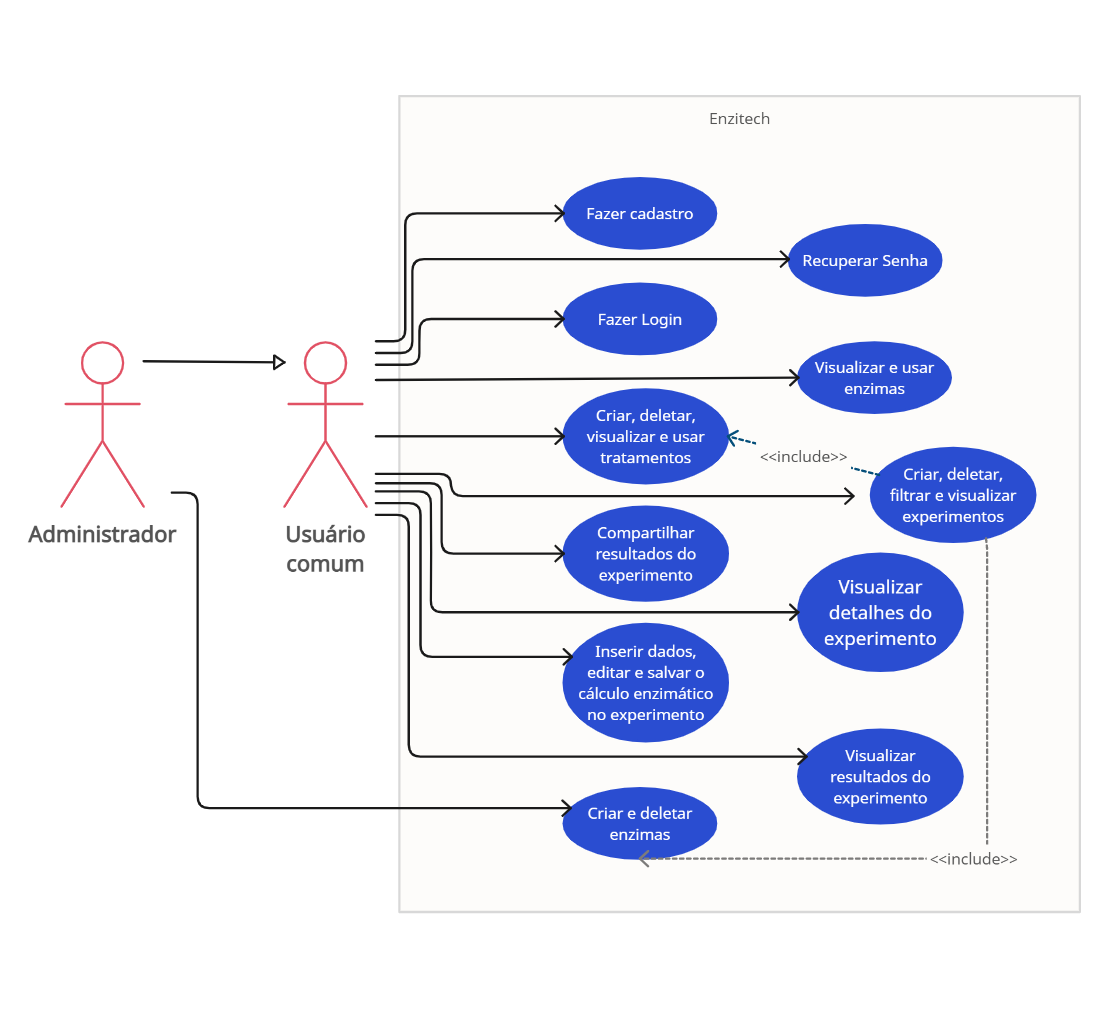
\includegraphics[width=\columnwidth]{images/use-cases-enzitech.png}
  \caption{Diagrama de Casos de Uso do sistema.}
  % \acsfont{Fonte: Autoria própria}
  \label{fig:use-cases-enzitech}
\end{figure}

Graças ao diagrama acima, é possível notar, de forma simples, que um usuário administrador possui um privilégio em comparação ao usuário comum: a criação e exclusão das enzimas, este Caso de Uso que ficou restrito à administração do sistema por ser compartilhada entre todos os usuários do Enzitech, podendo causar perdas de dados se sua alteração for realizada por um usuário comum, portando, surgiu a necessidade de diferenciar ambos os tipos de usuários no sistema e realizar estas validações para a disponibilização dessa \textit{feature}. 

\section{Protótipo}
\cite{warfel2009prototyping} destaca que os protótipos de baixa fidelidade são rápidos e baratos de criar, permitindo que os \textit{designers} testem e refinem rapidamente ideias iniciais. Já os protótipos de alta fidelidade, embora mais caros e demorados, podem ajudar a obter \textit{feedback} mais preciso e detalhado sobre o \textit{design} e a usabilidade do software.

Dentre as diversas reuniões do projeto, houve a discussão das funcionalidades para gerar um protótipo de baixa fidelidade, para possíveis refinamentos, antes da elaboração de um protótipo de alta fidelidade, que demanda mais tempo e esforço. Junto desse protótipo, foi idealizado a identidade visual e o nome oficial para o projeto, que passou a se chamar "Enzitech".

\begin{figure}[H]
\centering
  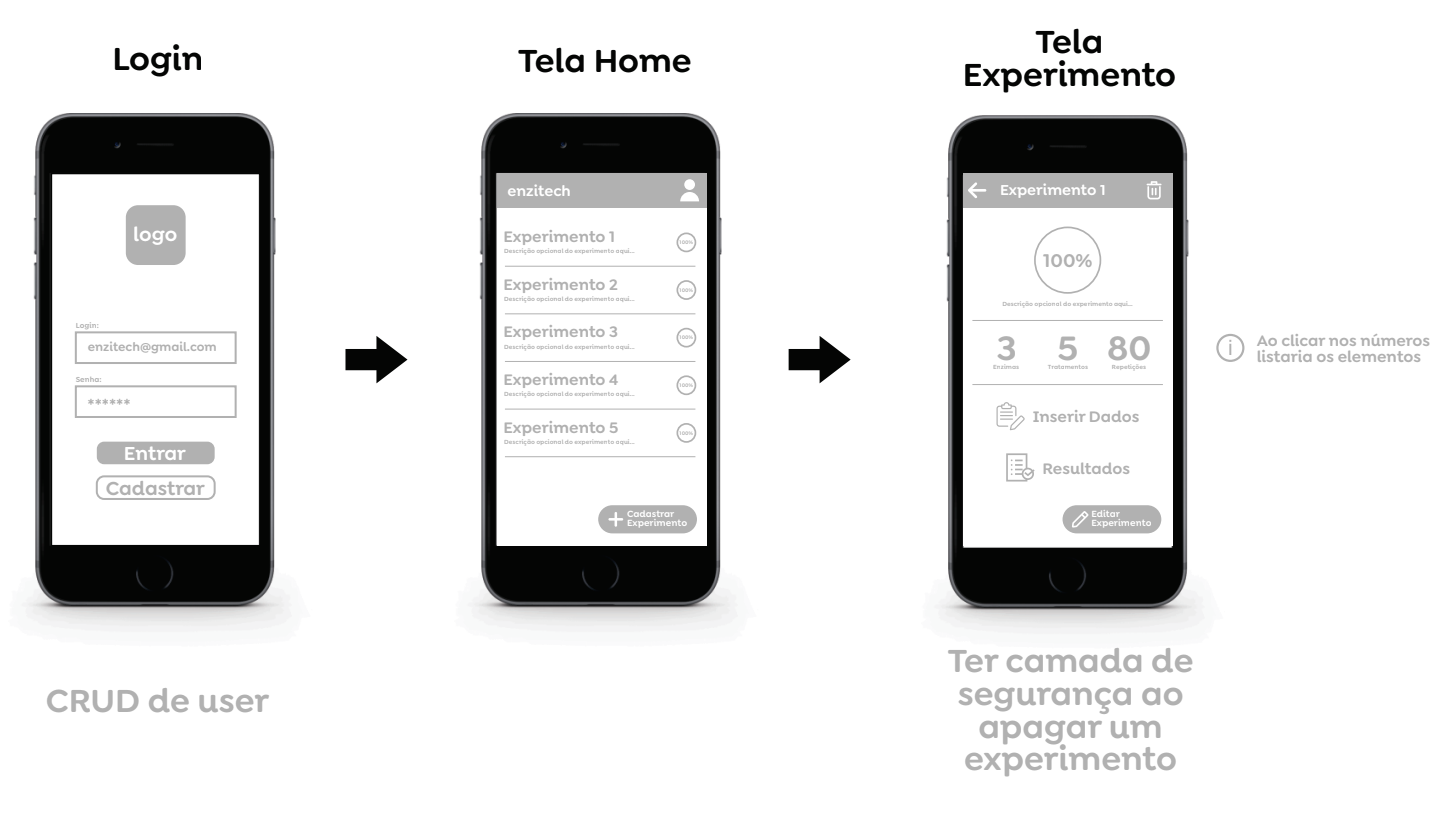
\includegraphics[width=\columnwidth]{images/prototipo_baixa.png}
  \caption{Parte do protótipo final de baixa fidelidade.}
  % \acsfont{Fonte: Autoria própria}
  \label{fig:prototipo_baixa}
\end{figure}

Como é possível ver na \figref{fig:prototipo_baixa}, o protótipo de baixa fidelidade trás o desenho das principais funcionalidades do sistema, além de dar uma ideia do layout final da aplicação.

\begin{figure}[H]
\centering
  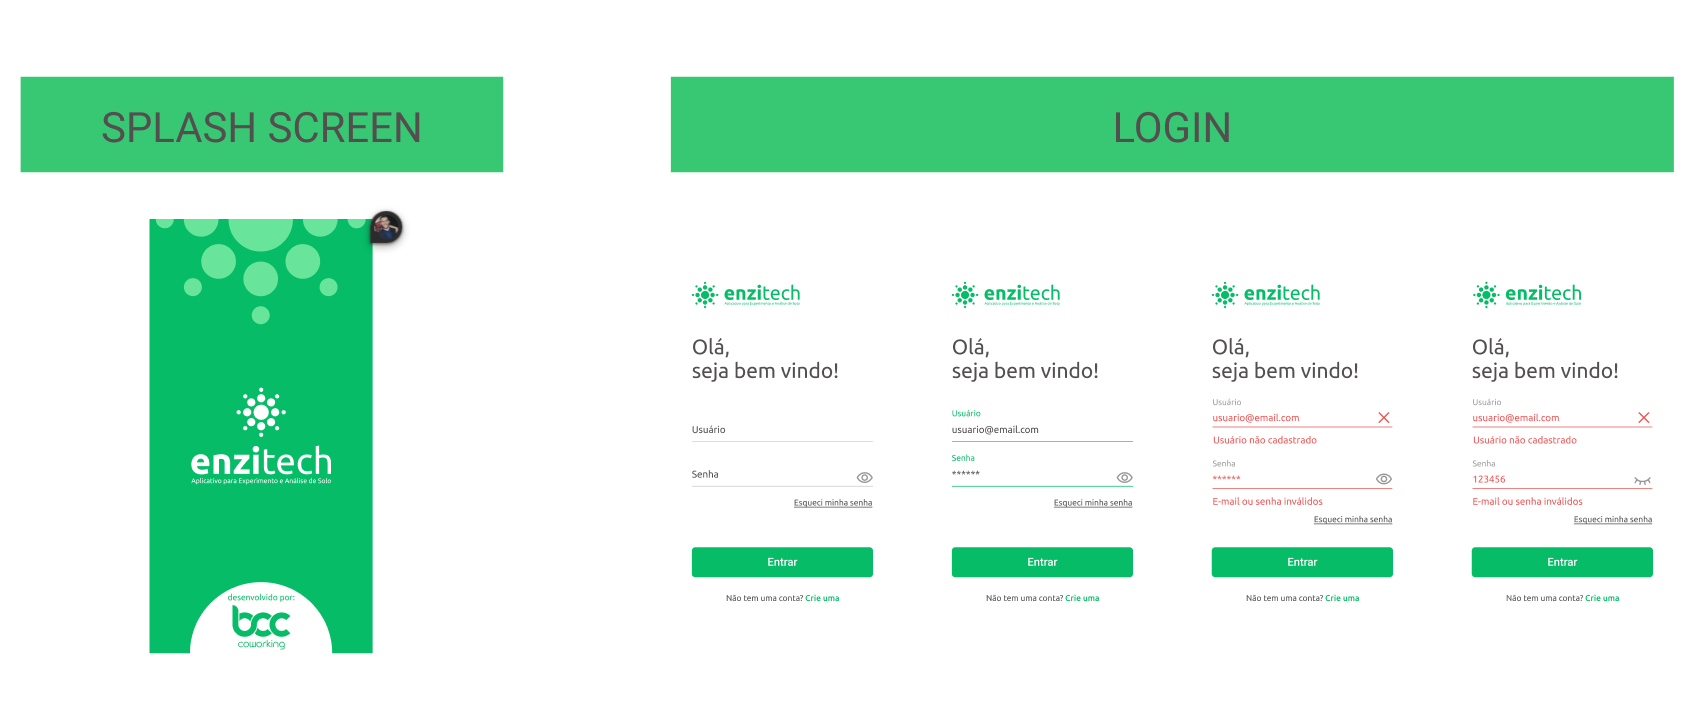
\includegraphics[width=\columnwidth]{images/exemplo_prototipo_alta.png}
  \caption{Parte do protótipo final de alta fidelidade.}
  % \acsfont{Fonte: Autoria própria}
  \label{fig:exemplo_prototipo_alta}
\end{figure}

Já nas \figref{fig:exemplo_prototipo_alta} e \figref{fig:prototipo_alta}, é possível verificar mais a fundo todo o \textit{design-system} aplicado, averiguar comportamentos das telas, fluxo de navegação, entre outras vantagens, trazendo uma versão muito mais refinada da aplicação, auxiliando o desenvolvimento e facilitando a visão do sistema para o cliente, onde antes era definido somente por Casos de Uso.

\begin{figure}[H]
\centering
  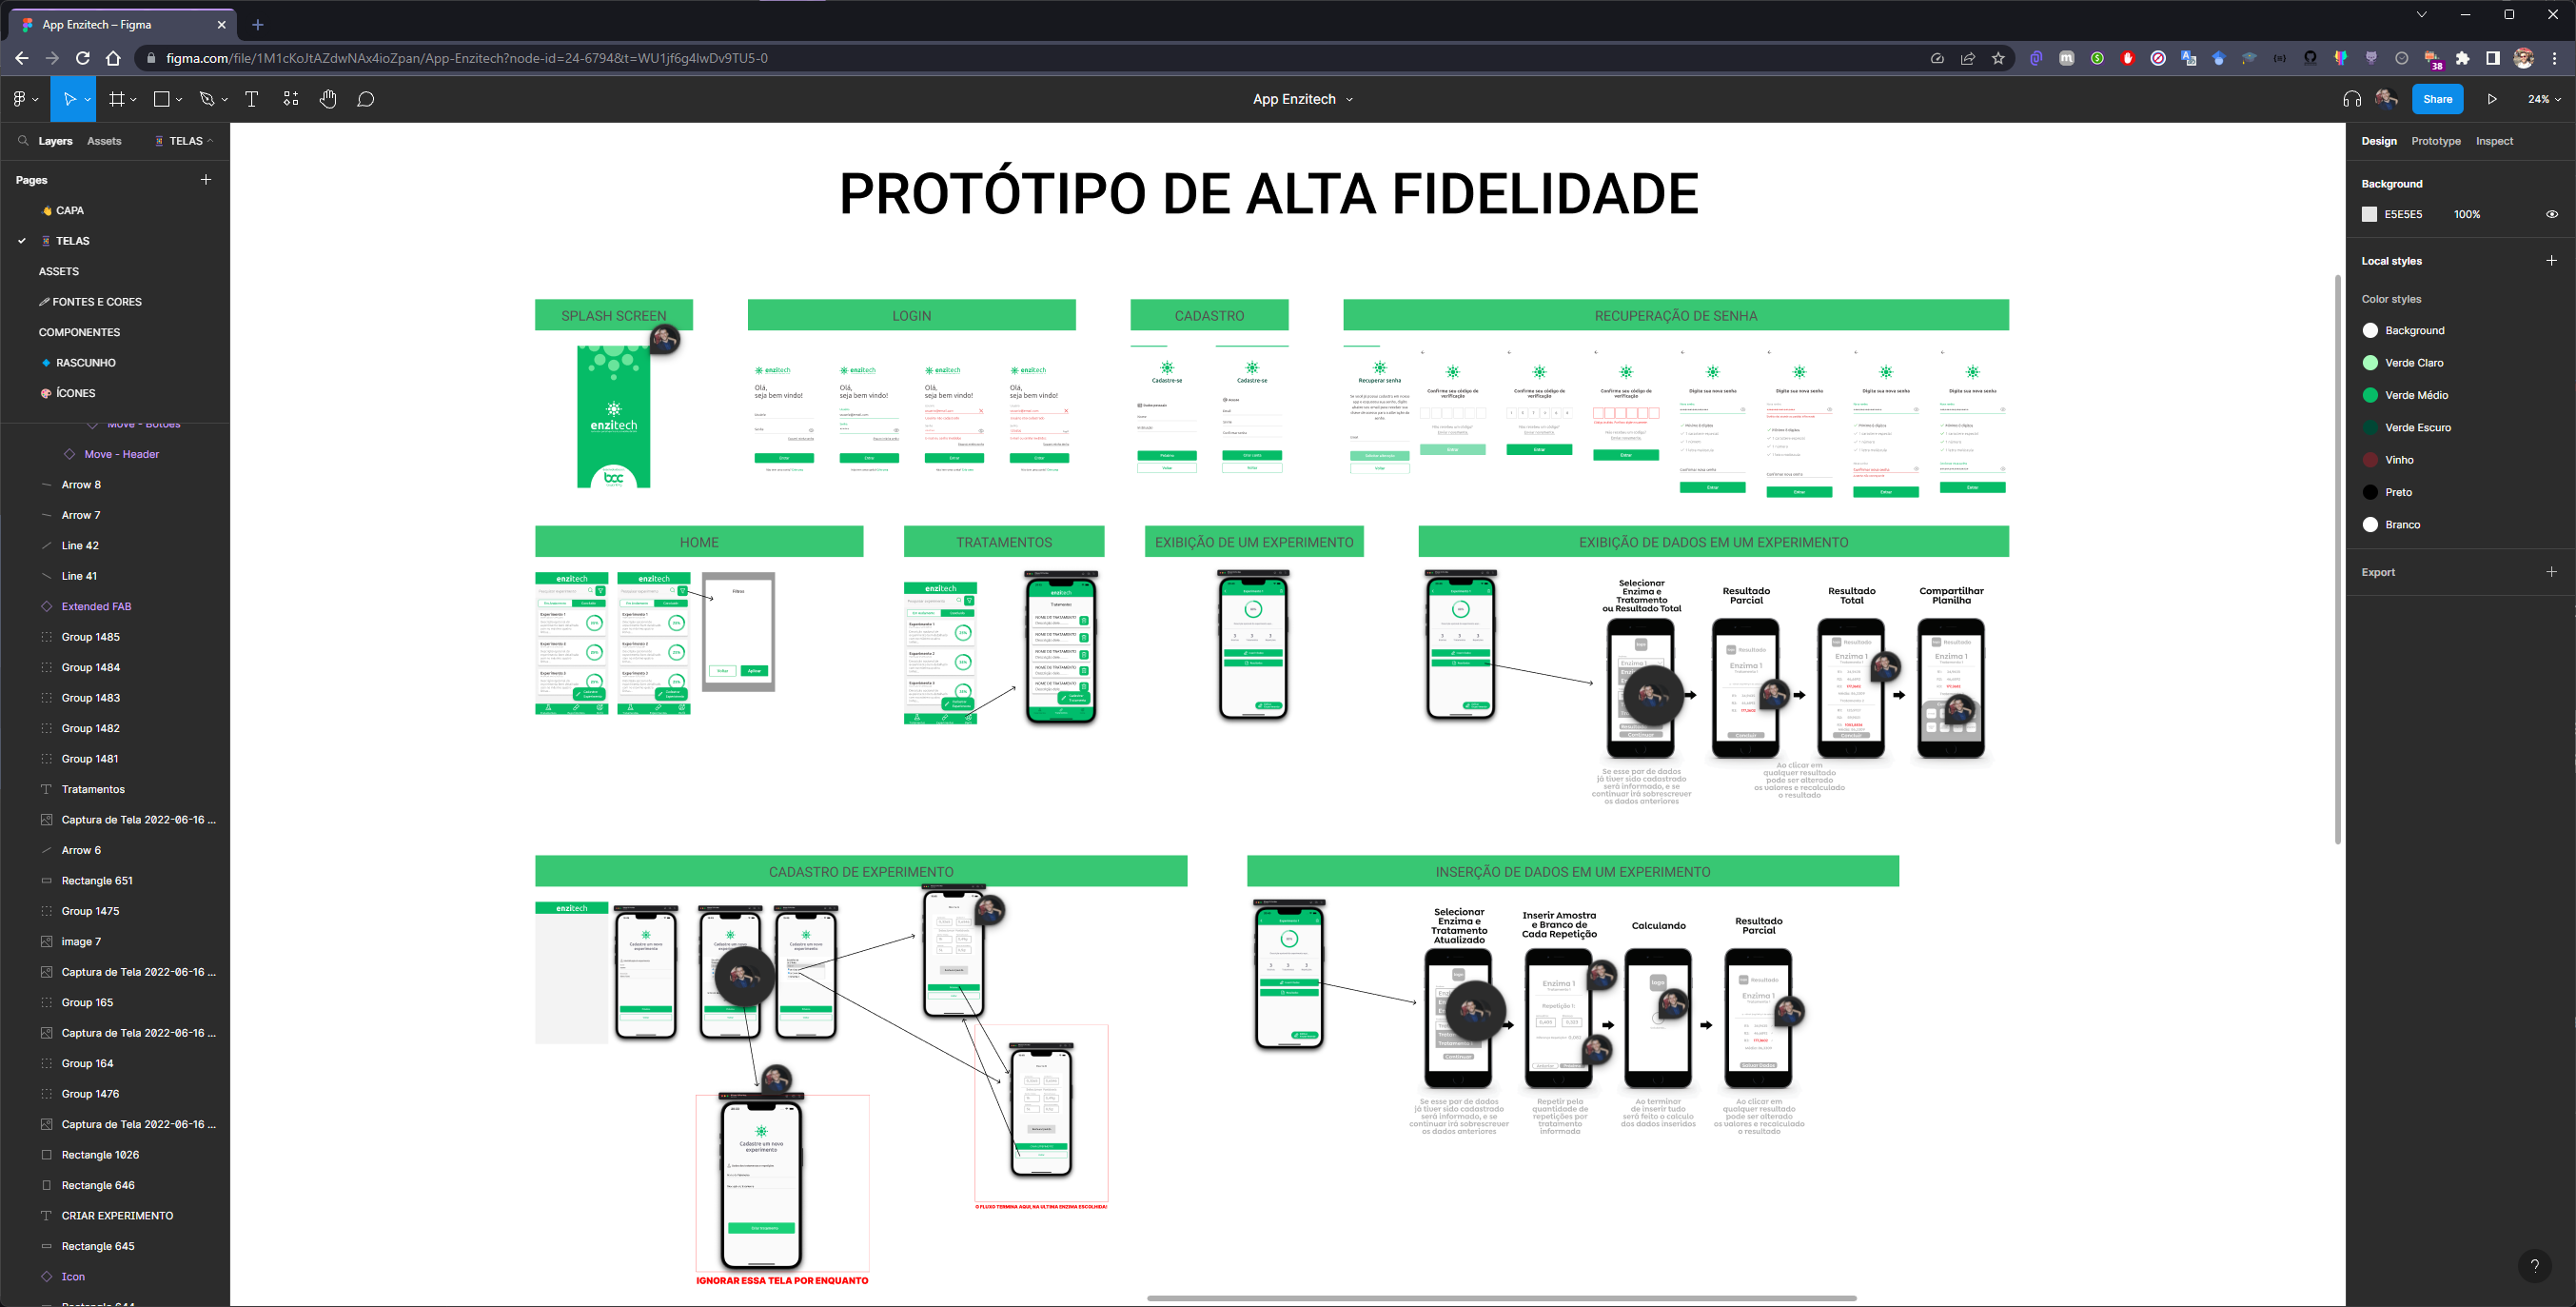
\includegraphics[width=\columnwidth]{images/prototipo_alta.png}
  \caption{Visão geral do protótipo final de alta fidelidade.}
  % \acsfont{Fonte: Autoria própria}
  \label{fig:prototipo_alta}
\end{figure}


\section{Tecnologias e ferramentas envolvidas}\label{sec:detalhes_tec}
Nesta seção, serão apresentados aspectos como tecnologias utilizadas, os passos necessários para a configuração do ambiente de desenvolvimento, a instalação do Flutter, ferramentas e bibliotecas utilizadas, integrações, gerenciamento de dependências, modelos de dados e o fluxo de trabalho.

\subsection{Instalação do Flutter}\label{ssec:instalacao_flutter}
% Instalação do Flutter e configuração do ambiente de desenvolvimento: Aqui, é importante descrever os passos necessários para instalar o Flutter e configurar o ambiente de desenvolvimento, incluindo a instalação do Android Studio, do emulador Android e da SDK do Android.
Antes de tudo, é necessário elucidar os requisitos para montar um ambiente de desenvolvimento voltado à criação de \acp{app} em Flutter, este \ac{sdk} está disponível nos principais \acp{so} de \acp{pc}, ChromeOS, macOS, Linux e Windows, sendo este último o escolhido como ambiente para o desenvolvimento desta aplicação, o qual será explicado o processo de instalação aqui.

De acordo com o site oficial\footnote{\label{flutter_install}Instalação do Flutter no Windows: \url{https://docs.flutter.dev/get-started/install/windows}}, para instalar e executar o Flutter, o ambiente de desenvolvimento deve atender a estes requisitos mínimos:
\begin{itemize}
   \item Windows 10 ou posterior (64 bits), baseado em x86-64;
   \item 1,64 GB de espaço livre no disco (não inclui espaço em disco para IDE/ferramentas);
   \item Ferramentas no ambiente do Windows:
   \begin{itemize}
     \item Windows PowerShell 5.0 ou mais recente (pré-instalado com o Windows 10);
     \item Git para Windows 2.x, com a opção "Use o Git no prompt de comando do Windows";
   \end{itemize}
 \end{itemize}

 Com todos os requisitos preenchidos, basta seguir o passo a passo detalhado como consta no site oficial\footref{flutter_install}.

\subsection{Instalação do Android Studio}\label{ssec:instalacao_android_studio}
Como consta no tutorial oficial\footref{flutter_install}, a instalação do Android Studio é essencial, porém neste passo, gosto de utilizar o \textit{JetBrains Toolbox App}\footnote{\label{toolbox}\textit{JetBrains Toolbox App}: \url{https://www.jetbrains.com/pt-br/toolbox-app/}}, que faz a instalação e futuras atualizações em poucos cliques. Após instalar o \textit{JetBrains Toolbox App}, basta achar o Android Studio e clicar em instalar.

\begin{figure}[H]
\centering
  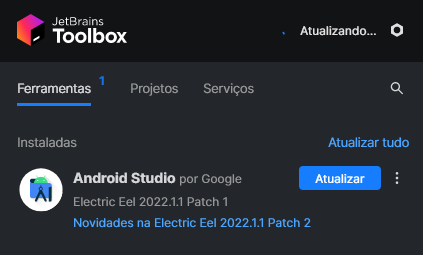
\includegraphics{images/toolbox.png}
  \caption{\textit{JetBrains Toolbox App}}
  % \acsfont{Fonte: Autoria própria}
  \label{fig:toolbox}
\end{figure}

Após instalado, é necessário abrir o Android Studio, fazer sua configuração inicial e configurar mais alguns passos, dentre eles, fazer a instalação de um emulador Android para utilizar no desenvolvimento, caso não queira utilizar um dispositivo físico, veja a seguir:
\begin{enumerate}
   \item Habilitar a "aceleração de VM" em sua máquina Windows;
   \item Na tela inicial do Android Studio, clique no ícone \textit{AVD Manager} e selecione \textit{Create Virtual Device…};
   \item Escolha uma definição de dispositivo e selecione "Avançar";
   \item Selecione uma ou mais imagens do sistema para as versões do Android que deseja emular e selecione Avançar. Uma imagem x86 ou x86\_64 é recomendada;
   \item Na aba de Performance do emulador, selecione Hardware - GLES 2.0 para habilitar a aceleração de hardware;
   \item Verifique se tudo está correto e selecione "Concluir";
   \item Por fim, basta executar o emulador e ele iniciará;
 \end{enumerate}

 Outro passo imprescindível é ativar as ferramentas \ac{sdk} necessárias para a compilação do projeto Flutter em um arquivo executável \textsc{.apk} para o Android, basta seguir este passo a passo:
 
 \begin{enumerate}
   \item Na tela inicial do Android Studio, clicar em \textit{File > Settings > Appearance \& Behavior > System Settings > \textit{Plugins}};
   \item Na aba \textit{Marketplace}, busque e instale os \textit{plugins} "Dart" e "Flutter";
   \item Nesta mesma tela, no menu lateral, clique em \textit{Appearance \& Behavior > System Settings > Android \ac{sdk}};
   \item Na aba \textit{\ac{sdk} Tools}, verifique se existem versões instaladas para \textit{Android SDK Build-Tools 34-rc2}, caso não, instale a correspondente à versão do Android escolhida na criação do emulador ou a do seu dispositivo físico;
   \item Ainda na aba \textit{\ac{sdk} Tools}, verifique se existe pelo menos uma versão instalada para \textit{Android SDK Command-line Tools}, caso contrário, instale a última versão disponível;
   \item Ainda na aba \textit{\ac{sdk} Tools}, verifique se o \textit{Android SDK Platform-Tools} está instalado, caso contrário, instale;
   \item Opcional: Ainda na aba \textit{\ac{sdk} Tools}, verifique se o \textit{Intel x86 Emulator Accelerator (HAXM installer)} está instalado, caso contrário, instale (esta ferramenta melhora a performance do emulador caso seu sistema suporte);
 \end{enumerate}
 
\subsection{Instalação do VSCode}\label{ssec:instalacao_vscode}
É possível seguir com o desenvolvimento no Android Studio, porém ele é um software que exige bastante processamento, o que pode "pesar" no sistema, principalmente se utilizado junto de um emulador Android, portanto, existe a possibilidade de utilizar o VSCode\footnote{\label{vscode}VSCode: \url{https://code.visualstudio.com/}} para seguir como software padrão de desenvolvimento, além disso, no VSCode é possível instalar uma grande quantidade de pacotes desenvolvidos pela comunidade que agilizam o desenvolvimento, para utilizar o VSCode basta instalá-lo pela loja do \ac{so}, no caso do Windows, a \textit{Microsoft Store} ou pelo site oficial\footref{vscode}. 

Após instalado e feito a configuração inicial, basta buscar e instalar os \textit{plugins} "Dart" e "Flutter", outros de sua preferência também podem ser instalados. Por fim, basta criar (seguindo o tutorial oficial\footnote{\label{create_app}Escreva seu primeiro aplicativo Flutter: \url{https://docs.flutter.dev/get-started/codelab}}) ou abrir um projeto Flutter já existente e começar a editar seu código.

\subsection{Ferramentas e bibliotecas de suporte}\label{ssec:ferramentas}
% Descrever as ferramentas e bibliotecas de suporte utilizadas no desenvolvimento, tais como o Visual Studio Code, o Dart DevTools, o Flutter DevTools e as bibliotecas de terceiros que podem ser utilizadas para ajudar no desenvolvimento da aplicação.
Além dos \acp{ide}, outras ferramentas foram utilizadas para o desenvolvimento do sistema, nesta subseção abordo brevemente cada uma e sua aplicação.
\subsubsection{Flutter DevTools}\label{sssec:flutter_devtools}
O DevTools\footnote{\label{dev_tools}DevTools: \url{https://docs.flutter.dev/development/tools/devtools/overview}} é um conjunto de ferramentas de desempenho e depuração para Dart e Flutter, vem integrado na instalação do Flutter e executa automaticamente na inicialização de \textit{debugging}, suas principais funções são:

 \begin{enumerate}
   \item Inspecionamento do layout da interface do usuário e o estado de um aplicativo Flutter;
   \item Diagnóstico de problemas de instabilidade no desempenho da interface do usuário em um aplicativo Flutter;
   \item Visualização de informações gerais de \textit{log} e diagnóstico sobre um aplicativo de linha de comando Flutter ou Dart em execução;
   % \item Entre outras funcionalidades;
 \end{enumerate}

\subsubsection{Postman}\label{sssec:postman}
O Postman\footnote{\label{postman}Postman: \url{https://www.postman.com/}} é uma ferramenta de teste de \ac{api} que permite aos desenvolvedores testar, documentar e compartilhar suas APIs. Com o Postman, é possível enviar solicitações \ac{http}, verificar as respostas da \ac{api}, criar scripts de teste automatizados e compartilhar coleções de solicitações com outras pessoas. A ferramenta é amplamente utilizada no desenvolvimento de software e pode ser integrada a outras ferramentas, como o Swagger\footnote{\label{swagger}Swagger: \url{https://swagger.io/}}, para tornar o processo de teste e documentação de \acp{api} mais eficiente.

\subsubsection{\textit{Packages} do pub.dev}\label{sssec:pubdev}
Os \textit{packages} do pub.dev\footnote{\label{pubdev}pub.dev: \url{https://pub.dev/}} são bibliotecas de código-fonte aberto, desenvolvidas por membros da comunidade Flutter, que podem ser utilizadas para implementar recursos em \acp{app} Flutter. Essas bibliotecas fornecem funcionalidades prontas para uso, como a integração com \acp{api}, manipulação de imagens, gerenciamento de estado, entre outras. 

Ao utilizar um \textit{package} do pub.dev, os desenvolvedores podem economizar tempo e esforço na implementação de funcionalidades comuns, além de poderem se beneficiar de contribuições e correções de \textit{bugs} feitas pela comunidade. Os \textit{packages} podem ser facilmente adicionados ao projeto por meio do arquivo \textsc{pubspec.yaml} e instalados por meio do comando \inlinecode{flutter pub get}.

